\documentclass[]{article}
\usepackage{lmodern}
\usepackage{amssymb,amsmath}
\usepackage{ifxetex,ifluatex}
\usepackage{fixltx2e} % provides \textsubscript
\ifnum 0\ifxetex 1\fi\ifluatex 1\fi=0 % if pdftex
  \usepackage[T1]{fontenc}
  \usepackage[utf8]{inputenc}
\else % if luatex or xelatex
  \ifxetex
    \usepackage{mathspec}
  \else
    \usepackage{fontspec}
  \fi
  \defaultfontfeatures{Ligatures=TeX,Scale=MatchLowercase}
\fi
% use upquote if available, for straight quotes in verbatim environments
\IfFileExists{upquote.sty}{\usepackage{upquote}}{}
% use microtype if available
\IfFileExists{microtype.sty}{%
\usepackage{microtype}
\UseMicrotypeSet[protrusion]{basicmath} % disable protrusion for tt fonts
}{}
\usepackage[margin=1in]{geometry}
\usepackage{hyperref}
\hypersetup{unicode=true,
            pdftitle={Software Failure and Reliability Assessment Tool: Report},
            pdfborder={0 0 0},
            breaklinks=true}
\urlstyle{same}  % don't use monospace font for urls
\usepackage{longtable,booktabs}
\usepackage{graphicx,grffile}
\makeatletter
\def\maxwidth{\ifdim\Gin@nat@width>\linewidth\linewidth\else\Gin@nat@width\fi}
\def\maxheight{\ifdim\Gin@nat@height>\textheight\textheight\else\Gin@nat@height\fi}
\makeatother
% Scale images if necessary, so that they will not overflow the page
% margins by default, and it is still possible to overwrite the defaults
% using explicit options in \includegraphics[width, height, ...]{}
\setkeys{Gin}{width=\maxwidth,height=\maxheight,keepaspectratio}
\IfFileExists{parskip.sty}{%
\usepackage{parskip}
}{% else
\setlength{\parindent}{0pt}
\setlength{\parskip}{6pt plus 2pt minus 1pt}
}
\setlength{\emergencystretch}{3em}  % prevent overfull lines
\providecommand{\tightlist}{%
  \setlength{\itemsep}{0pt}\setlength{\parskip}{0pt}}
\setcounter{secnumdepth}{0}
% Redefines (sub)paragraphs to behave more like sections
\ifx\paragraph\undefined\else
\let\oldparagraph\paragraph
\renewcommand{\paragraph}[1]{\oldparagraph{#1}\mbox{}}
\fi
\ifx\subparagraph\undefined\else
\let\oldsubparagraph\subparagraph
\renewcommand{\subparagraph}[1]{\oldsubparagraph{#1}\mbox{}}
\fi

%%% Use protect on footnotes to avoid problems with footnotes in titles
\let\rmarkdownfootnote\footnote%
\def\footnote{\protect\rmarkdownfootnote}

%%% Change title format to be more compact
\usepackage{titling}

% Create subtitle command for use in maketitle
\newcommand{\subtitle}[1]{
  \posttitle{
    \begin{center}\large#1\end{center}
    }
}

\setlength{\droptitle}{-2em}
  \title{Software Failure and Reliability Assessment Tool: Report}
  \pretitle{\vspace{\droptitle}\centering\huge}
  \posttitle{\par}
  \author{}
  \preauthor{}\postauthor{}
  \date{}
  \predate{}\postdate{}


\begin{document}
\maketitle

\section{Tab 1: Select, Apply, and Analyze
Data}\label{tab-1-select-apply-and-analyze-data}

\subsection{Sample of the updated data different
formats:}\label{sample-of-the-updated-data-different-formats}

\begin{longtable}[]{@{}rrr@{}}
\caption{First ten points of the input data}\tabularnewline
\toprule
FN & IF & FT\tabularnewline
\midrule
\endfirsthead
\toprule
FN & IF & FT\tabularnewline
\midrule
\endhead
1 & 3 & 3\tabularnewline
2 & 30 & 33\tabularnewline
3 & 113 & 146\tabularnewline
4 & 81 & 227\tabularnewline
5 & 115 & 342\tabularnewline
6 & 9 & 351\tabularnewline
7 & 2 & 353\tabularnewline
8 & 91 & 444\tabularnewline
9 & 112 & 556\tabularnewline
10 & 15 & 571\tabularnewline
\bottomrule
\end{longtable}

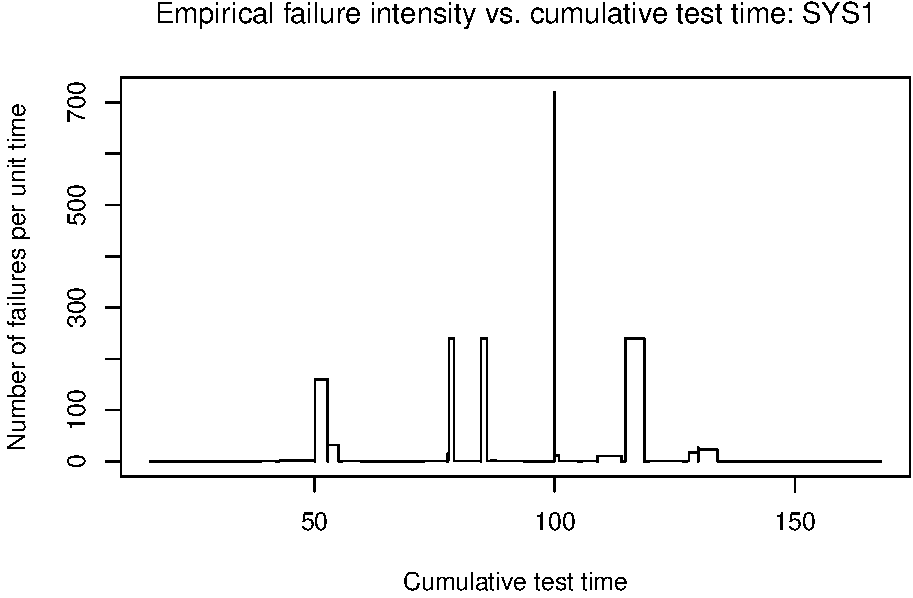
\includegraphics{C:/Users/Shekar/Desktop/SFRAT_~1/Reports/SFRATR~1/figure-latex/unnamed-chunk-5-1.pdf}

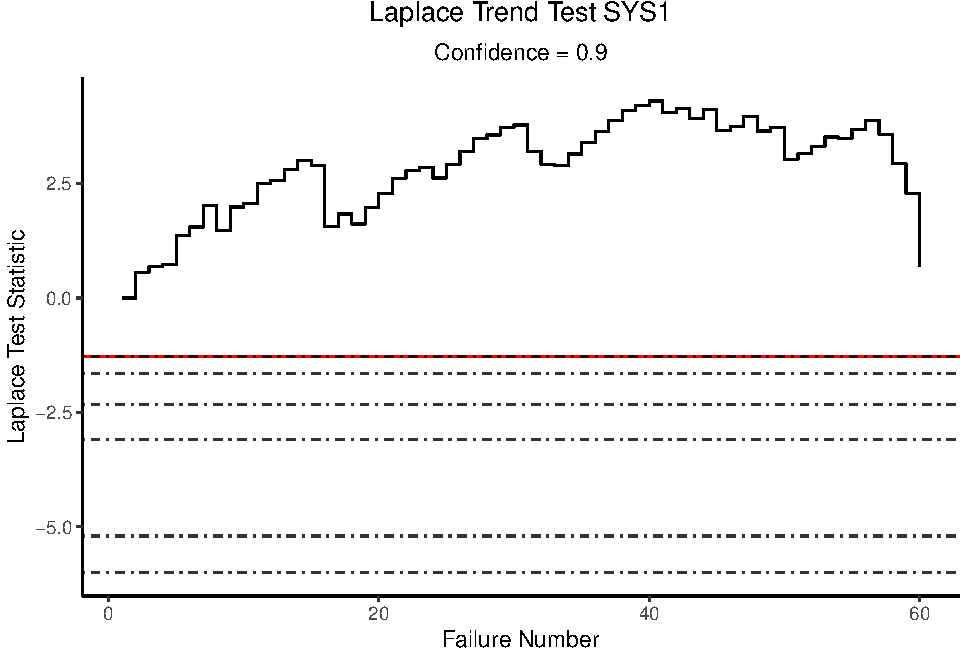
\includegraphics{C:/Users/Shekar/Desktop/SFRAT_~1/Reports/SFRATR~1/figure-latex/unnamed-chunk-6-1.pdf}

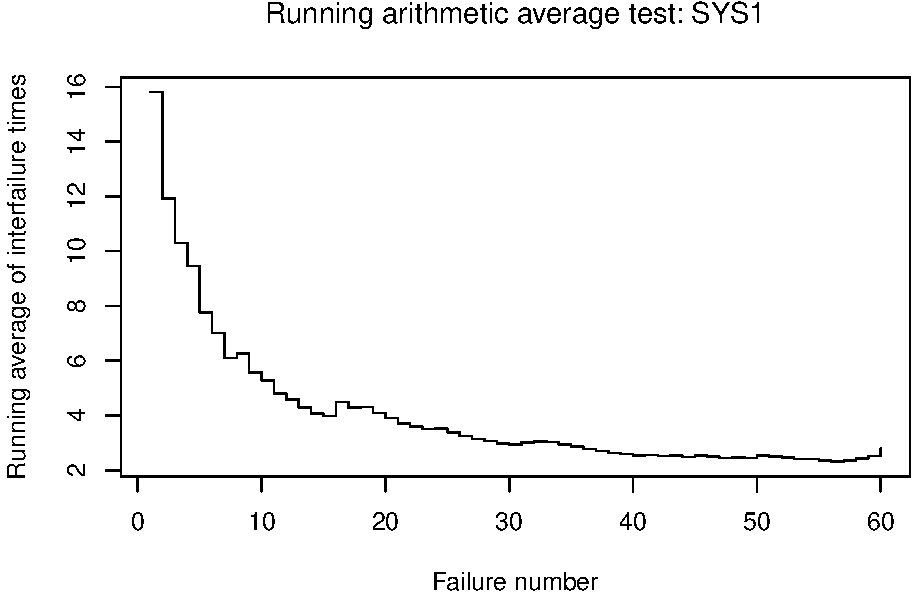
\includegraphics{C:/Users/Shekar/Desktop/SFRAT_~1/Reports/SFRATR~1/figure-latex/unnamed-chunk-7-1.pdf}

\subsection{The Laplace test is the default trend test, which possesses
a statistical interpretation and allows the user to specify a confidence
level between 0 and 1 to quantify a desired level of significance that
the data exhibits (or does not exhibit) reliability growth. Decreasing
trend indicates reliability growth and the red line indicates the user
specified significance
level.}\label{the-laplace-test-is-the-default-trend-test-which-possesses-a-statistical-interpretation-and-allows-the-user-to-specify-a-confidence-level-between-0-and-1-to-quantify-a-desired-level-of-significance-that-the-data-exhibits-or-does-not-exhibit-reliability-growth.-decreasing-trend-indicates-reliability-growth-and-the-red-line-indicates-the-user-specified-significance-level.}

\includegraphics{C:/Users/Shekar/Desktop/SFRAT_~1/Reports/SFRATR~1/figure-latex/unnamed-chunk-8-1.pdf}

\subsection{The running arithmetic average, computes and plots a running
average of the times between failures. A plot exhibiting a positive
slope indicates that the times between failures are increasing,
suggesting reliability growth during
testing.}\label{the-running-arithmetic-average-computes-and-plots-a-running-average-of-the-times-between-failures.-a-plot-exhibiting-a-positive-slope-indicates-that-the-times-between-failures-are-increasing-suggesting-reliability-growth-during-testing.}

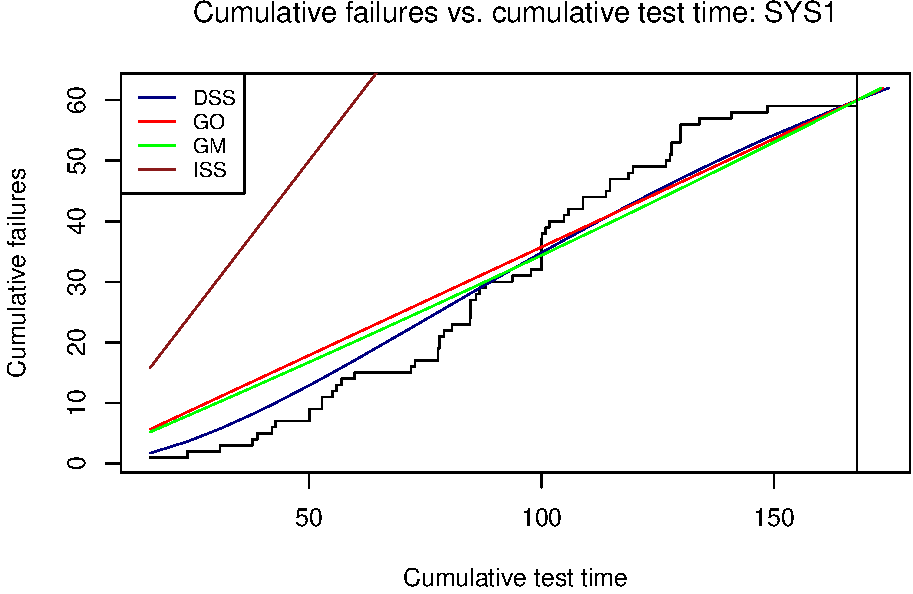
\includegraphics{C:/Users/Shekar/Desktop/SFRAT_~1/Reports/SFRATR~1/figure-latex/unnamed-chunk-9-1.pdf}

\section{Tab2: Set Up and Apply
Models}\label{tab2-set-up-and-apply-models}

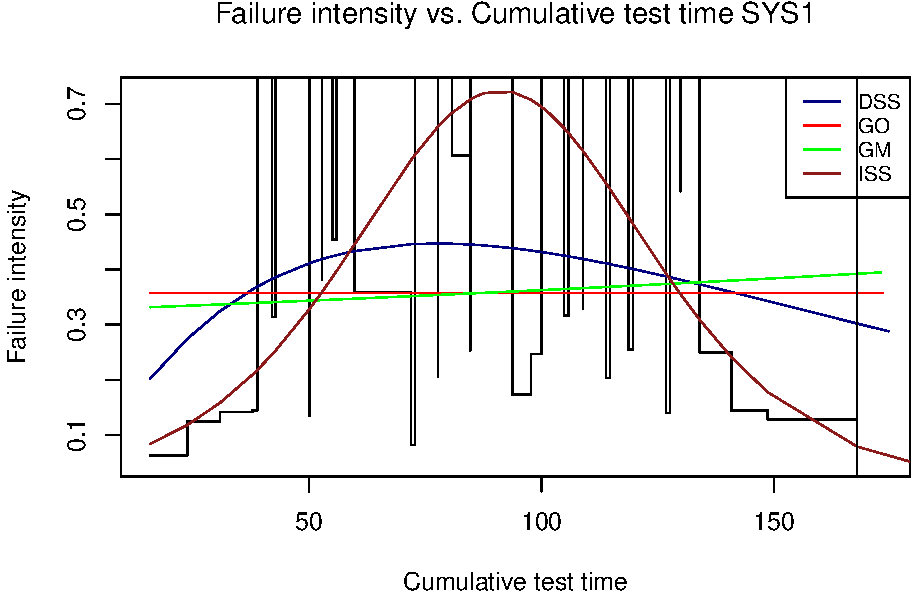
\includegraphics{C:/Users/Shekar/Desktop/SFRAT_~1/Reports/SFRATR~1/figure-latex/unnamed-chunk-11-1.pdf}

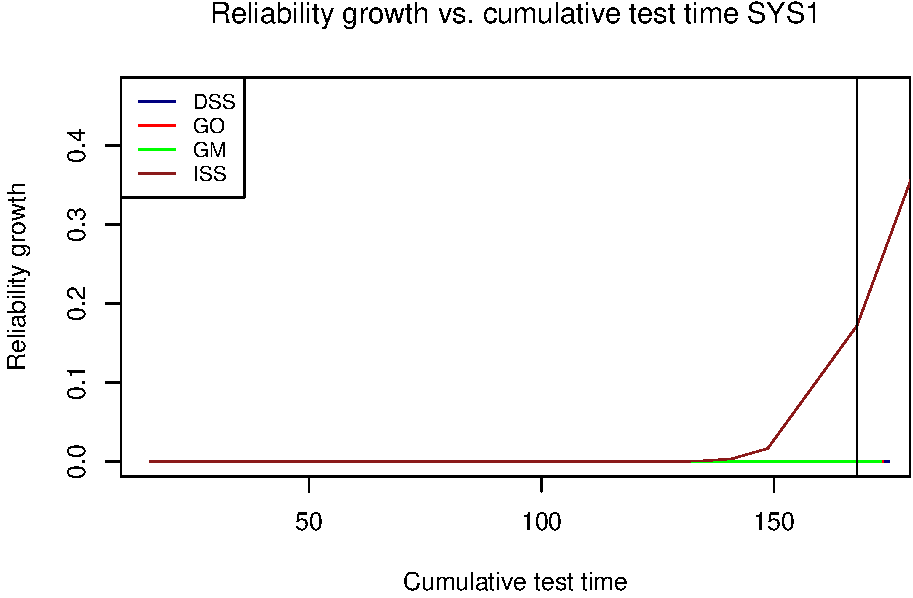
\includegraphics{C:/Users/Shekar/Desktop/SFRAT_~1/Reports/SFRATR~1/figure-latex/unnamed-chunk-12-1.pdf}

\includegraphics{C:/Users/Shekar/Desktop/SFRAT_~1/Reports/SFRATR~1/figure-latex/unnamed-chunk-13-1.pdf}

\includegraphics{C:/Users/Shekar/Desktop/SFRAT_~1/Reports/SFRATR~1/figure-latex/unnamed-chunk-14-1.pdf}

\section{Tab3: Query Model Results}\label{tab3-query-model-results}

\begin{longtable}[]{@{}llll@{}}
\toprule
& Time to achieve specified reliability & Expected number of failures &
Expected time to N failure\tabularnewline
\midrule
\endhead
DSS & R = 0.9 achieved & 0.246856262199799 & NA\tabularnewline
GO & 8263.13681952821 & 0.00235313039055995 &
4591.28466949961\tabularnewline
JM & 91142.2377161945 & 0.00223287121590943 &
4869.80650205625\tabularnewline
GM & 153028.269493869 & 0.00466173473881781 &
2170.03088926781\tabularnewline
Wei & 66732.9968495319 & 0.0043270671047253 &
2353.05254648438\tabularnewline
\bottomrule
\end{longtable}

\section{Tab4: Evaluate Models}\label{tab4-evaluate-models}

\subsection{Smaller values of AIC and PSSE values are
preferred.}\label{smaller-values-of-aic-and-psse-values-are-preferred.}

\begin{longtable}[]{@{}lrr@{}}
\toprule
& AIC & PSSE\tabularnewline
\midrule
\endhead
DSS & 2075.146 & 296.34925\tabularnewline
GO & 1953.613 & 23.07129\tabularnewline
JM & 1950.534 & 19.60037\tabularnewline
GM & 1937.034 & 84.32708\tabularnewline
Wei & 1938.161 & 74.94496\tabularnewline
\bottomrule
\end{longtable}


\end{document}
